\section{Model}

The input data is a collection of cascades $\mathcal{C}=\{S_m\}_{m=1}^M$. 
A cascade $S=\{(t_k, u_k)|u_k\in U, t_k\in R^+ \text{~and~}
k=1,\dots,N\}$ is a sequence of propagations ascendingly ordered by time, where $U$ refers to 
user set in cascade. The $k$-th propagation is recorded
as a tuple $(t_k, u_k)$ referring to pair of activated time and user.
Let the history $\mathcal{H}_k$ be the list of activated time and user pairs up
to the $k$-th propagation. The objective of sequence modeling in cascade dynamics is to
formulate the conditional probability probability of next propagation
$p((t_k, u_k)|\mathcal{H}_k)$.

\subsection{Background}

Firstly, we introduce RNN in cascade dynamics modeling. RNN is a feed-forward
neural network, which can be used to generate a cascade by $N$ steps
sequentially.
At each step $k$, the $k$-th propagation vectorized in $x_k$ as input is fed
into hidden units of RNN by nonlinear transformation $f$, jointly with the outputs from the last hidden units, updating the hidden state
$h_k=\textit{RNN}(x_k,h_{k-1})$. The representation of hidden state $h_k$ can be
considered as embedding of the $k$-th propagation, and the output is trained to predict the
next propagation $x_{k+1}$ given $h_k$. In other words, we use RNN to
maximize the likelihood probability of cascade,
\begin{equation*}
p(S) = \prod_{k=1}^N p((t_{k+1}, u_{k+1})|\mathcal{H}_k) = \prod_{k=1}^N
p((t_{k+1}, u_{k+1})|h_k).
\end{equation*}
The conditional probability $p((t_{k+1}, u_{k+1})|h_k)$ can be
formalized by a joint probability on both next activated time and user, such as,
\begin{equation*}
\label{eq:cond_prob}
\begin{aligned}
p((t_{k+1}, u_{k+1})|h_k)=& p(t_{k+1}|h_{k}) \cdot
p(u_{k+1}|h_{k}) \\
= & f(t; h_{k}) \cdot \text{softmax}(g(h_k)),
\end{aligned}
\end{equation*}
where $g$ is a non-linear function.
The function $f(t;h_{k})$ refers to a temporal point process
parameterized by $h_{k}$,
\begin{equation*}
\begin{aligned}
& f(t; h_{k})=\lambda(t)\exp\left(-\int_{t_k}^t\lambda(\tau)d\tau\right) \\
&\textit{s.t.~~} \lambda(t) = \exp(wt+U^{(t)}h_k), 
\end{aligned}
\end{equation*}
where $w$ is a scalar and $U^{(t)}$ is a parameter matrix.
% we define conditional probability of next propagation by a
% joint probability on next activated time and user, such as:
% \begin{equation*}
% \label{eq:cond_prob}
% \begin{aligned}
% p(x_{k+1}|\mathcal{H}_k)=& p(t_{k+1}|x_{k}, T_{k}, s_{k}) \cdot p(u_{k+1}|x_{k}, T_{k}, s_{k}) \\
% = & f(t; x_{k}, T_{k}, s_{k}) \cdot \text{softmax}(g(x_{k}, T_{k}, s_{k})).
% \end{aligned}
% \end{equation*}
% The function $f(t;x_{k},T_{k},s_{k})$ refers to a temporal point process
% parameterized by $x_{k},T_{k},s_{k}$,
% \begin{equation*}
% \begin{aligned}
% & f(t; x_{k}, T_{k},
% s_{k})=\lambda(t)\exp\left(-\int_{t_k}^t\lambda(\tau)d\tau\right) \\
% &\textit{s.t.~~} \lambda(t) = \exp(wt+W^{(t)}x_k+U^{(t)}t_{k-1}+Z^{(t)}s_k) 
% \end{aligned}
% \end{equation*}
Based on sufficient observed cascades, RNN
can find an optimal solution for the above equation
in a huge functional space, avoiding the bias on diffusion
model and limits on diffusion network.
Thus, RNN can be a promising and flexible method to capture the complex
propagation patterns in cascade dynamics modeling. 

% \subsection{Background}
% % \noindent{\textbf{CDM based on RNN:}}
% Firstly, we introduce RNN 
% % as an eventwise modeling method 
% in cascade dynamics modeling. A cascade $S=\{x_i|x_i=(t_i, u_i), u_i\in U
% \text{~and~} t_i\in R^+\}_{i=1}^N$ is a set of propagations ascendingly ordered
% by time, where $U$ refers to all possible activated users in cascade. The
% $i$-th propagation $x_i$ is recorded as a tuple $(t_i, u_i)$ referring to
% activated time and user respectively. Then, RNN can be used to simulate the
% generation of propagations by $N$ steps sequentially. At each step $k$, the $k$-th
% propagation are fed into hidden units of RNN by nonlinear transformation $f$,
% jointly with the outputs from the last hidden units, updating the hidden state
% $h_k=f(x_i,h_{k-1})$. The representation of hidden state $h_k$ can be considered
% as embedding of the $k$-th propagation, and the output is
% trained to predict the next propagation $x_{k+1}$ given $h_k$. In other words,
% we use RNN to maximize the likelihood probability of cascade,
% \begin{equation}
% \label{eq:likelihood}
% p(S)=\prod_{k=1}^N p(x_{k+1}|h_k).
% \end{equation}
% % The embeddings of propagations $E(x_i)$ are given as inputs
% % to RNN. At each step $k$, the network updates its hidden state $h_k=f(E(x_i),
% % h_{k-1})$, where $f$ is certain nonlinear functions.  
% % In RNN, the input to an encoder is an activation sequence
% % $S=\{x_i|x_i=(t_i, u_i)\}_{i=1}^N$ asendingly ordered by time. The activation
% % $x_i$ is recorded as a tuple $(t_i, e_i)$ referring to activated time and activated
% % user respectively. The embeddings of activation are given as inputs to RNN. At
% % each step $k$, the network updates 
% % The current inputs are fed
% % into hidden units by nonlinear transformation, jointly with the outputs from the
% % previous hidden units, and then generate the next activation in cascade. The
% % representation of hidden units can be recognized as the event embedding
% % to the corresponding inputs. 
% Based on sufficient observed cascades, RNN
% can find an optimal solution for Eq.~(\ref{eq:likelihood})
% in a huge functional space, avoiding the limits of prior knowledge on
% diffusion model.
% Thus, RNN can be a promising method to capture the complex propagation patterns in cascade
% dynamics modeling. 

However, RNN suffers crossing dependency problem caused by tree-structured
propagations in cascade, shown in Fig.~\ref{fig:mot}. One of the possible
solutions is to construct a pooling layer above the hidden
units at each $k$ step in order to build the direct dependence between the
next propagation and all previous propagation embeddings,
i.e., $p(x_{k+1} | \text{pooling}(h_1,\ldots,h_k))$. The simplest way of pooling can
be formalized as
\begin{equation}
\label{eq:pooling_frame}
s_k=\sum_{i=1}^k \alpha_{k,i} h_i \text{,~~~~~s.t.~} \sum_{i=1}^k
\alpha_{k,i}=1,
\end{equation}
where the weight $\alpha_{k,i}$ refers to the proportion of dependence between
next propagation and the $i$-th propagation embedding. Mean pooling and max
pooling are two popular choices for setting weights which takes the mean or element-wise
max of all hidden states. However, these two methods still ignore the structure
information in cascades.
% Mean pooling and max pooling
% are two popular choices for setting weights which takes the mean or
% element-wise max of all hidden states. 
% In this way, the generation of next activation
% can depend on any historical embedding instead of transitive dependency.
Intuitively, the weights can be settled according to the cascade tree, yet we
can hardly obtain the tree structure, even given the social relationships. Next
we propose attention mechanism to implement the pooling layer. 

\begin{figure}[t]
\centering
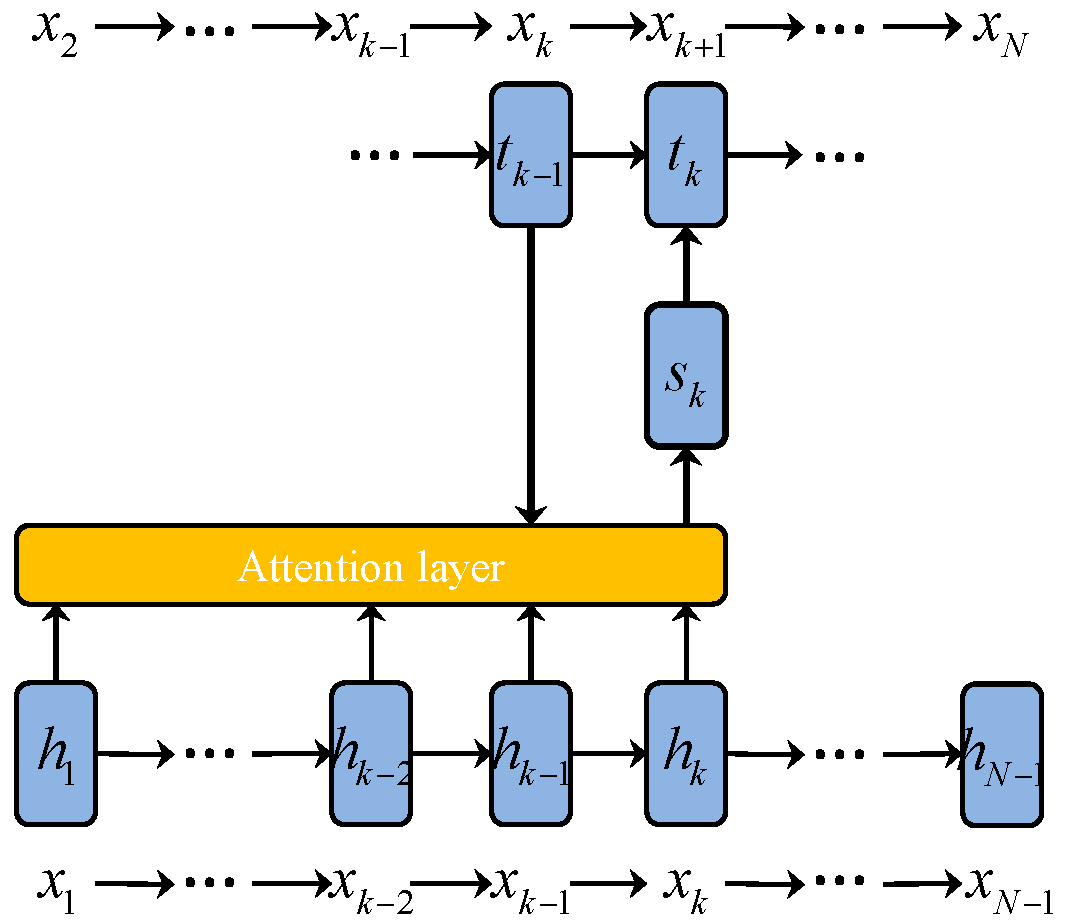
\includegraphics[width=0.45\textwidth]{figs/cyanrnn_framework.png}
\caption{The architecture of CYAN-RNN. The figure presents the case when
modeling the generation of the $(k+1)$-th propagation. The sequence at bottom is
the observed propagations and the sequence at top is the predictive
propagations. The blue rectangles refer to representations of hidden units.
% in source sequence, attention layer, and hidden units in target sequence. 
The yellow rectangle is a general form of attention function
$s_k=\textit{AttentionFunc}(t_{k-1}, \{h_1,\ldots,h_k\})$.}
\label{fig:cyrnn_frame}
\end{figure}

\subsection{Attention Mechanism}
Attention mechanism is orginally used in neural machine translation (NMT).
% firstly proposed by Bahdanau et.al~\cite{bahdanau2014neural}. 
In the senario of attention-based NMT, the target words are translated by the
words in source sequence and attention mechanism can automatically learn the alignment
between source words and target words.
For modeling cascade dynamics, the source sequence will be the observed
cascade.
The each element in target sequence is the following propagation corresponded to
propagation in source sequence.
There remains one problem when applying attention mechanism in cascade dynamics
modeling: the target is the next propagation in source
sequence, thus the alignments between source and target sequence need to be dynamically updated
when the context $\{h_1,\ldots,h_k\}$ is growing along with the proceeding
propagations.

% the both source and target sequence originate from the same cascade
% and 
% the alignments between source and target sequence need to be dynamically
% updated when the context $\{h_1,\ldots,h_k\}$ is growing along with the
% proceeding propagations.
% we conduct the
% observed cascade as the source sequence. The each propagation in target sequence
% is the following propagation corresponding to the propagation in source
% sequence. 
% the words in source sequence need to be
% aligned to the words in target sequence. 
% Attention-based RNN can adaptively
% learn the alignment between source and target sequences. 
% However, there remains two problems when applying attention mechanism in
% cascade dyanmics modeling:
% 1) The both source and target sequences originate from the same cascade; 
% Only source sequence can be observed in a cascade, thus we need to
% construct targets.
% 2) The size of
% alignments in attention mechanism needs to be updated when the context
% $\{h_1,\ldots,h_k\}$ is growing along with the proceeding propagations.

We propose a dynamic attention mechanism for CYAN-RNN.
% for cascade dynamics with attention-based RNN.
The proposed architecture is shown in Fig.~\ref{fig:cyrnn_frame}. 
According to the architecture, we rewrite the conditional probability of next
propagation
\begin{equation*}
\begin{aligned}
p((t_{k+1}, u_{k+1})|&\mathcal{H}_k)=p((t_{k+1}, u_{k+1})|x_k, T_k, s_k)\\
&=f(t; x_{k}, T_{k}, s_{k}) \cdot \text{softmax}(g(x_{k}, T_{k}, s_{k})).
\end{aligned}
\end{equation*}
% by a joint probability on next activated time and user, such as:
% \begin{equation*}
% \label{eq:cond_prob}
% \begin{aligned}
% p(x_{k+1}|\mathcal{H}_k)=& p(t_{k+1}|x_{k}, T_{k}, s_{k}) \cdot p(u_{k+1}|x_{k}, T_{k}, s_{k}) \\
% = & f(t; x_{k}, T_{k}, s_{k}) \cdot \text{softmax}(g(x_{k}, T_{k}, s_{k})).
% \end{aligned}
% \end{equation*}
% The function $f(t;x_{k},T_{k},s_{k})$ refers to a temporal point process
% parameterized by $x_{k},T_{k},s_{k}$,
% \begin{equation*}
% \begin{aligned}
% & f(t; x_{k}, T_{k},
% s_{k})=\lambda(t)\exp\left(-\int_{t_k}^t\lambda(\tau)d\tau\right) \\
% &\textit{s.t.~~} \lambda(t) = \exp(wt+W^{(t)}x_k+U^{(t)}t_{k-1}+Z^{(t)}s_k) 
% \end{aligned}
% \end{equation*}
% where $g$ is an objective function defined the joint probability
% on both activated time and user. 
% Here we use the objective function
% formalized in RMTPP~\cite{DuKDD2016}.
% We propose CYAN-RNN for cascade dynamics modeling, applying a dynamic
% attention mechanism to solve the crossing dependency problem. The architecture
% of CYAN-RNN is shown in Fig.~\ref{fig:cyrnn_frame}. In CYAN-RNN, we conduct the
% observed cascade as the source sequence. The each propagation in target sequence
% is the following propagation corresponding to the propagation in source
% sequence. 
% % The target sequence is the set of following propagations corresponding to the
% % propagations in source sequence.
% % copy of source sequence, 
% % is the copy of source sequence and shift one
% % , shifting one step of the copy backwards. 
% The objective is to
% jointly predict the next propagation and learn the alignment of dependence
% between the next propagation and historical propagation embeddings. 
% % As to the target
% % sequence, we copy the source sequence and then shift one step of the copy backwards. 
% According to the architecture, we define each conditional probability in
% Eq.~(\ref{eq:likelihood}) as:
% \begin{equation}
% \label{eq:cond_prob}
% p(x_{k+1}|x_1,\ldots,x_k)=g(x_k, t_{k}, s_{k}),
% \end{equation}
% where $g$ is an objective function defined the joint probability
% on both activated time and user. Here we use the objective function
% formalized in RMTPP~\cite{DuKDD2016}.
% \begin{equation}
% \label{eq:rmtpp}
% \begin{aligned}
% g(x_k,t_{k},s_{k})&=p(u_{k+1}|t_k, s_k, x_k)\cdot p(t_{k+1}| t_k, s_k, x_k)\\
% &=\text{softmax}(t_k, s_k, x_k)\cdot
% \lambda(t_{k+1})\exp\left(-\int_{t_k}^{t_{k+1}}\lambda(\tau)d\tau \right)
% \end{aligned}
% \end{equation}
The decoding state $T_k$ for the $k$-th step in target
sequence is computed by
\begin{equation}
\label{eq:target_embedding}
T_k = f(x_k, T_{k-1}, s_k),
\end{equation}
where 
% subscript in exponential function is the index of vector.   
$f$ is
a nonlinear activation function, which can be either a \textit{tanh} or
a \textit{sigmoid} function. The context vector $s_k$ is calculated by
Eq.~(\ref{eq:pooling_frame}) where the weights $\alpha_{k,.}$ 
% in proposed attention mechanism 
is updated by the growth context
$\{h_1,\ldots,h_k\}$ and $T_{k-1}$. The weight $\alpha_{k,i}$ is formalized as
\begin{equation}
\label{eq:alpha}
\alpha_{k,i}=\frac{\exp(e_{k,i})}{\sum_{j=1}^k \exp(e_{k,j})},
\end{equation}
where
\begin{equation}
\label{eq:score}
e_{k,i}=a(T_{k-1}, h_i)=v^T\tanh(W^{(a)} T_{k-1}+U^{(a)} h_i)
\end{equation}
scores how well the dependence between the $i$-th propagation
embedding and the output at the $k$-th step, and $W^{(a)}$ and $U^{(a)}$ are the
parameter matrices. The implementation of attention mechanism in proposed model
is briefly represented in Fig.~\ref{fig:att}.

% Given a collection of cascades $\mathcal{C}=\{S_m\}_{m=1}^M$, we suppose that
% each cascade is independent on each other. As a result, the logarithmic
% likelihood of a set of cascades is the sum of logarithmic likelihood of individual cascade.
% In this way, the negative logarithmic likelihood of the set of cascades can be
% estimated as
% \begin{equation}
% \mathcal{L}(\mathcal{C})=-\sum_{m=1}^M \sum_{k=1}^{N_m} \left[
% g(x_k^{(m)}, t_{k}^{(m)}, s_{k}^{(m)}) \right], 
% \end{equation}
% and we can learn parameters of the proposed model by minimizing the negative
% logarithmic likelihood.
%  $\arg \min_\theta \mathcal{L}(\mathcal{C})$, where $\theta$ is the
% parameter set in the model. 
With the attention mechanism, the alignments $\alpha_{k,.}$ can be directly
updated through the cost function, thus exploit an expected representation
$s_k$ over all historical propagation embeddings for each step $k$.

% The weights in proposed attention
% mechanism $s_k=\sum_{i=1}^k \alpha_i h_i$   
% The context vector $s_k$ is a representation, calculated in
% Eq.~(\ref{eq:pooling_frame}).

% to model cascade dynamics, the learned weights in
% attention and also infer the tree structure of propagations. The architecture of CYAN-RNN is shown in
% Fig.~\ref{fig:framework}.
% We firstly conduct the observed cascade as the source sequence.
% Then we copy the cascade and then shift one step of the copy backwards as the target
% sequence. 
 
\begin{figure}[ht!]
\centering
\subfigure[] {
\label{fig:att}
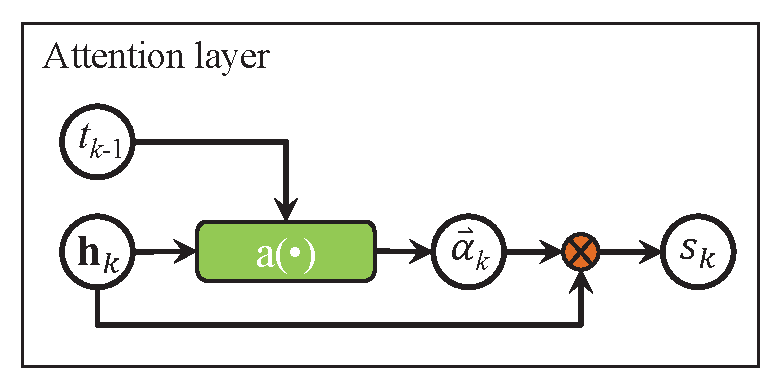
\includegraphics[width=0.35\textwidth]{figs/att.eps}
}
\subfigure[] {
\label{fig:cov}
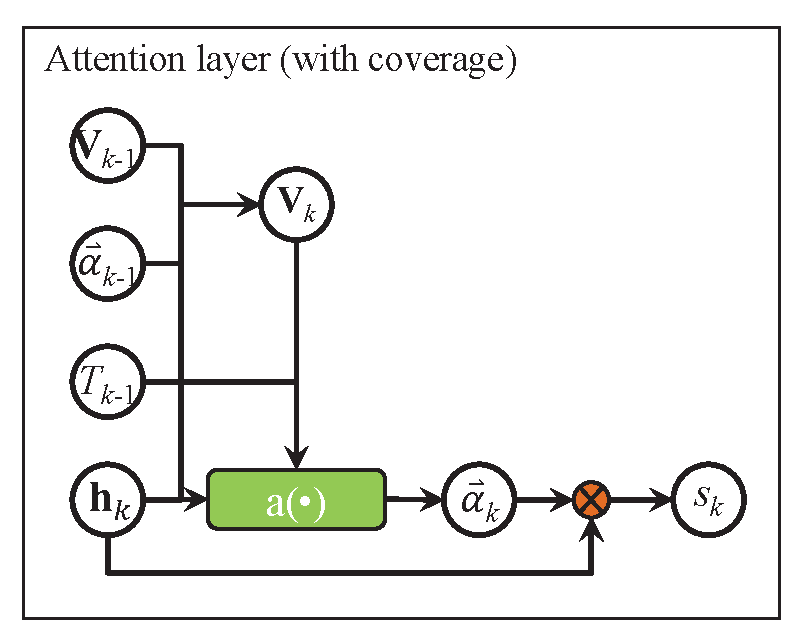
\includegraphics[width=0.35\textwidth]{figs/cov.eps}
}
\caption{Two kinds of implementation on attention layer. (a) The attention
mechanism applied in CYAN-RNN; (b) The attention mechanism with coverage applied
in CYAN-RNN (cov). Note that $\textbf{h}_k=(h_1,\ldots,h_k)$ is matrix assembled by all
historical propagation embeddings at step $k$, and
$\textbf{V}_k=(V_1,\ldots,V_k)$ is a coverage martix containing all coverage
vectors at step $k$.}
\end{figure}

\subsection{Coverage}
\label{sec:coverage}

Furthermore, we propose coverage to lead alignments focused more on 
recent propagation embeddings, following the similar perference of users'
interests in real system. The example is shown in
Fig.~\ref{fig:mot}.
If the user $u_1$ is an influential user and her propagation is key to the
cascade, the propagation triggered by $u_4$ may depend more on the 1st
propagation embedding triggered by $u_1$, achieving a larger alignment
weight than the 2nd propagation embedding. But the $u_4$ is the
immediate successor of $u_2$ in cascade tree instead of $u_1$ in practice.
In this way, the 1st propagatoin embedding is \emph{over-dependent} and the
2nd propagation embedding is \emph{under-dependent} when modeling the
generation of the 4th propagation.

% In this
% way, embedding of $(t_1, u_1)$ is over-dependent and embedding of $(t_2, u_2)$ is under-dependent when modeling
% the generation of the 4th propagation.
%  
% Although CYAN-RNN is proposed to better model cascade dynamics in consideration
% of crossing dependency problem, the proposed model still suffer
% \emph{over-dependent} and \emph{under-dependent} problems in
% attention mechanism.
% As the exmaple shown in Fig.~\ref{fig:mot}, if the user $u_1$ is an influential
% user and her propagation is key to the cascade, the propagation activated by
% $u_4$ may perfer to depend more on embedding of $(t_1, u_1)$ instead of $(t_2, u_2)$.
% In this way, embedding of $(t_1, u_1)$ is over-dependent and embedding of $(t_2,
% u_2)$ is under-dependent when modeling the generation of the 4th propagation. In
% practice, it is a common phenomenon that users may have a higher probability
% activated by recent propagation than past ones and we also conduct experiments
% to illustrate it (see section~\ref{sec:exp}).

The two problems are caused by memoryless of dynamic attention mechanism.
Inspired by linguistic coverage model, we formulate the general form of
coverage in cascade dynamics modeling, keeping historical alignments so as to
release the over-dependent and under-dependent problems. The $k$-th step of coverage is defined as
\begin{equation}
\label{eq:cov}
V_{k,i}=f\left(V_{k-1, i}, \alpha_{k-1,i}, t_{k-1}, h_i\right).
\end{equation}
Remarkably, as the increasing context and alignments, $V_{k,k}$ and
$\alpha_{k,k}$ have no corresponding values in $V_{k-1,.}$ and
$\alpha_{k-1,.}$. Instead we fill up with zero in our work. 
% Compared with $V_{k,i}$, $V_{k-1,i}$ 
At each step $k$, the $k$-th coverage serves an additional input to the
attention mechanism, providing complementary information of that how about the
dependencies of propagation embeddings are in the past. The rewritten
alignment calculation in Eq.~(\ref{eq:score}) by coverage can be
formalized~\footnote{
% The formalization is determined by the incremental length
% of alignment weights. 
If we use the last coverage $V_{k-1,.}$ instead of
$V_{k,.}$ (like~\cite{tu2016modeling}) to update $e_{k,.}$ at each step $k$, 
we will lose certain coverage information and cause unbalanced
calculation on $k$-th propagation embedding, proved by our preliminary
experiments.} as
\begin{equation}
\label{eq:att_cov}
\begin{aligned}
e_{k,i} &= a(T_{k-1}, h_i, V_{k,i}) \\
& = v^T\tanh(W^{(a)} T_{k-1}+U^{(a)} h_i+Z^{(a)} V_{k,i}),
\end{aligned}
\end{equation}
where $W^{(a)}$, $U^{(a)}$ and $Z^{(a)}$ are parameter matrices. We expect that
the alignment weights would be focus more on recent propagation embeddings. The
expectation will be validated in section~\ref{sec:exp}.

\subsection{Length of Dependence}
Practically, a cascade may last long and the propagation length would be huge,
causing an extreme computation cost when applying dynamic attention mechanism
proposed in CYAN-RNN. According to perference of users' interests on recent
propagations, we consider a hyper-parameter, \emph{length of dependence}
$l$, limiting the size of alignments so that the predictive task can only
depend on last $l$ propagations. Empirically, we set $l=200$ at most cases.

% Thus, the attention mechanism only need to calculate the
% $\max (k, t)$ historical event embeddings 
